\documentclass[10pt,twocolumn,letterpaper]{article}

\usepackage{icb}
\usepackage{times}
\usepackage{epsfig}
\usepackage{graphicx}
\usepackage{amsmath}
\usepackage{url}
\usepackage{amssymb}

\DeclareMathOperator*{\argmin}{arg\,min}

% Include other packages here, before hyperref.

% If you comment hyperref and then uncomment it, you should delete
% egpaper.aux before re-running latex.  (Or just hit 'q' on the first latex
% run, let it finish, and you should be clear).
%\usepackage[pagebackref=true,breaklinks=true,letterpaper=true,colorlinks,bookmarks=false]{hyperref}

%\icbfinalcopy % *** Uncomment this line for the final submission

\def\icbPaperID{****} % *** Enter the IJCB Paper ID here
\def\httilde{\mbox{\tt\raisebox{-.5ex}{\symbol{126}}}}


% Pages are numbered in submission mode, and unnumbered in camera-ready
\ificbfinal\pagestyle{empty}\fi
\begin{document}

%%%%%%%%% TITLE
\title{Effects of using pre-compressed data for compression studies in iris recognition}

\author{First Author\\
Institution1\\
Institution1 address\\
{\tt\small firstauthor@i1.org}
% For a paper whose authors are all at the same institution,
% omit the following lines up until the closing ``}''.
% Additional authors and addresses can be added with ``\and'',
% just like the second author.
% To save space, use either the email address or home page, not both
\and
Second Author\\
Institution2\\
First line of institution2 address\\
{\tt\small secondauthor@i2.org}
}






\maketitle
\thispagestyle{empty}

%%%%%%%%% ABSTRACT
\begin{abstract}
   The ABSTRACT is to be in fully-justified italicized text, at the top
   of the left-hand column, below the author and affiliation
   information. Use the word ``Abstract'' as the title, in 12-point
   Times, boldface type, centered relative to the column, initially
   capitalized. The abstract is to be in 10-point, single-spaced type.
   Leave two blank lines after the Abstract, then begin the main text.
   Look at previous ICB abstracts to get a feel for style and length. 
\end{abstract}

%%%%%%%%% BODY TEXT
\section{Introduction}

Iris recognition \cite{BBurge13a,Rathgeb12e} is one of the most deployed biometric
modalities, standardized by the International Civil Aviation
Organization (ICAO) for use in future passports, and one of
the technologies in the Unique Identification Authority of
India's (UID) Aadhaar project to uniquely identify Indian
citicens. However, the increasing market saturation of
biometric instead of conventional access control methods
raises the need for efficient means to store such data. The
International Organization for Standardization (ISO)
specifies iris biometric data to be recorded and stored in (raw)
image form (ISO/IEC FDIS 19794-6), rather than in extracted
templates (e.g. iris-codes). On the one hand, such
deployments benefit from future improvements (e.g. in
feature extraction stage) which can be easily incorporated
without re-enrollment of registered users. On the other hand,
since biometric templates may depend on patent-registered
algorithms, databases of raw images enable more
interoperability and vendor neutrality \cite{Rathgeb12e}. These facts
motivate detailed investigations and optimisations of image
compression on iris biometrics in order to provide an efficient
storage and rapid transmission of biometric records.
Furthermore, the application of low-powered mobile sensors
for image acquisition, e.g. mobile phones, raises the need for
reducing the amount of transmitted data.

The certainly most relevant standard for compressing
image data relevant in biometric systems is the ISO/IEC
19794 standard on Biometric Data Interchange Formats
where in the most recently published version (ISO/IEC FDIS
19794-6), only JPEG2000 is included for lossy compression.
JPEG2000 has also been recommended for various
application scenarios and standardised iris images (IREX
records) by the NIST Iris Exchange  (IREX
\url{http://iris.nist.gov/irex/}) program. The ANSI/NIST-ITL
1-2011 standard on ``Data Format for the Interchange of
Fingerprint, Facial \& Other Biometric Information'' (former
ANSI/NIST-ITL 1-2007) also supports only JPEG2000 for
applications tolerating lossy compression.

As a consequence, according to the importance of this issue, many studies comparing and optimising lossy compression techniques for iris imagery 
may be found in the litarature. Since the CASIA iris datasets have been very popular among researchers ever since their establishment,
many papers dealing with compression have been relying the (extended) CASIA V1.0 dataset, including also first IREX investigations 
\cite{BRakshit07a,BIves08a,Matschitsch07a,Haemmerle09a,Konrad09a} (apart from other examples using the ICE 2005 dataset 
% noch V1: BIves05a,Konrad09b,Kostmajer09a,BRakshit06a,
\cite{BDaugman08a,BIves10a}).
	
	However, since it has been pointed out \cite{BPhilips07a} that the CASIA V1.0 dataset exhibits manipulated pupil areas and should therefore not 
	be used any further in experimentation, compression researchers moved to other (and more recent, more challenging etc.) datasets, e.g. 
	the CASIA V3.0 \cite{Horvath11b,Rathgeb12e}, 
	the CASIA V4.0 \cite{BTuba12a}, the Bath \cite{BIves08a,BPardamean12a}, and the UBIRIS.v1 \cite{Haemmerle09a,BCarneiro11a} datasets, respectively.
	While the images of CASIA V1.0 and ICE 2005 are given in uncompressed format, images in CASIA V3.0, CASIA V4.0, UBIRIS and Bath datasets are
	provided as JPEG (the first three) or JPEG2000 (the latter) lossy compressed data, respectively. Therefore, any compression experiments conducted
	on these datasets operate on pre-compressed data. 
	
	This fact has not been ignored entirely -- for example, in \cite{Rathgeb12e}, preparatory JPEG compression experiments with uncompressed data reveal that 
	slighly pre-compressed data leads to better recognition performance due to denoising effects and thus experiments with pre-compressed data are assessed to
	be unproblematic. The same argument is used for JPEG2000 pre-compressed data \cite{BPardamean12a} based on the results in \cite{BIves08a}.
	However, eventual artifacts resulting from recompression effects are not accounted for in these considerations. Recompression artifacts arise in case
	data is compressed twice (or multiple times) with lossy compression schemes, where artifacts from the first compression step (termed pre-compression)
	are aggravated by the second compression step.
	
	Two different types of such effects may be distinguished: First, intra-recompression, where the same compression scheme is used several times, whereas
	in inter-recompression different codecs are used in the different compression steps. For example, using JPEG pre-compressed data and applying
	JPEG XR and JPEG2000 \cite{Horvath11b} or JPEG2000 and fractal compression \cite{BCarneiro11a} is eventually prone to inter-recompression
	artifacts, while the application of JPEG to JPEG pre-compressed data \cite{BTuba12a,Rathgeb12e} can be prone to intra-recompression artifacts.
	
	While next to nothing can be found on the issue of inter-recompression artifacts in the general compression literature, 
	intra-recompression artifacts are better investigated, at least in the case of lossy JPEG compression. Soon after the establishment of
	the JPEG standard \cite{Pennebaker93a}, it was found that JPEG recompression artifacts arise and do not follow a linear behaviour \cite{Chan92a}.
	Extensive experiments in this direction can also  be found in \cite{Kumar11a}, and following these obversations, requantisation-based schemes have been
	suggested for JPEG, reducing recompression artifacts considerably \cite{Bauschke03a}. Recently, the identification of images which underwent 
	JPEG double compression (i.e. JPEG intra-recompression) has been a hot topic in image forensics \cite{Sencar12a}.
	
	Taking all these facts together, it gets clear, that recompression artifacts may impact experimental results with respect to biometric recognition
	performance, an issue, that has been neglected so far. In this paper, we systematically investigate eventual intra- and inter-recompression effects 
	in an experimental study
	for iris recognition. Given the importance of JPEG in the area (as the CASIA V3.0/V4.0 and UBIRIS.v1 datasets are only available in this format), we 
	focus on JPEG pre-compressed data. In our experiments, we compare iris recognition, iris segmentation, and general purpose image quality metrics applied
	to single compressed vs. recompressed (i.e. JPEG pre-compressed) iris image data. In Section 2, we ...... 
	

\section{Test data generation and compression scheme}
\label{section:comprScheme}
We investigate whether using already pre-compressed data as a basis for image compression performance rating in iris biometric systems produces a different outcame than if truly uncompressed data has been used for the same rating process. Using pre-compressed data, this means when compression is applied, a pre-compressed image $I_p$ is compressed a second time, hence we denote this process as \emph{double-compression} resulting in an image $I_d$. When compressing a truly uncompressed image $I_u$, which was read directly from the sensor, we denote this as \emph{single-compression} with a resulting image $I_s$. Since experiments are typically carried out on a data set with more than one image, we denote $I_u^{(k)}, I_p^{(k)}, I_s^{(k)}, I_d^{(k)} \in \mathbb{R}^{w \times h}$ as the $k^{th}$ image with width $w$ and height $h$ in the particular data sets. Furthermore, we denote $s(F) \in \mathbb{N}$ with $F \sim{I \in \mathbb{R}^{w \times h}}$ as a function that returns the file size of the file $F$ storing an image $I \in \mathbb{R}^{w \times h} $. Since common lossy compression algorithms also employ lossless compression methods on the pixel data before writing to a file, $F$ is loosely linked to the contained pixel data $I$. For simplicity, we denote $s(I)$ as the file size of the file $F$ encoding the pixel values of an image $I$. $c_{m}(I, q)$ with $q \in \mathbb{N}$ defines the compression of an image $I$ with a particular method $m$ using the quality parameter $p$. In terms of this paper we use the values $m \in \{jpg, jxr, j2k\}$, where 
\begin{itemize}
	\item $jpg$ corresponds to the well-known (ISO/IEC IS 10918-1) DCT-based image compression method \cite{jpg},
	\item $j2k$ corresponds to the wavelet-based image compression standard (ISO/IEC IS 15444-1), which can operate at higher compression ratios \cite{j2k} and
	\item $jxr$ corresponds to a compression standard based on Microsoft’s HD Photo, which is specified in (ISO/IEC IS 29199-2) \cite{jxr}.  
\end{itemize}

%TODO: Consider: Do I have to specify which methods we used (Matlab JxrEncApp) to come up with the images? As it is a standard, this shouldn't be necessary, because everything operates the same anyway?!

For rating an image §I§'s compression effectiveness, we define the compression ratio $cr$ between an uncompressed image $I_u$ and a compressed image $I_c$ as 
\begin{equation}
cr(I_u, I_c) = \frac{s(I_u)}{s(I_c)} \quad \text{with} \quad I_c \in \{I_d, I_s\}
\end{equation}

For the later described experiments, images are compressed to a target compression ratio $cr_t \in \mathbb{R}$. All three compression methods take one parameter $q \in \mathbb{N}$ only, which controls the image quality but not the file size of the output image. Hence it is not possible to set this parameter in a way to meet a certain target compression ratio $cr_t$. Due to the limited universe of the quality parameters, the target compression ratio $cr_t$ cannot be achieved exactly, but a parameter optimization can be done, so that $cr_t \approxeq cr(I_u^{(k)}, I_c^{(k)})$. We propose an algorithm to compress a data set of $K$ uncompressed images $I_u$ using a particular method $m$ to achieve a certain compression ratio $cr_t := \gamma$ with $\gamma \in \mathbb{R}$ , e.g. $cr_t := 50$ in a way that the compression ratio of each image is met as close as possible. This process, illustrated in Fig. \ref{fig:comprScheme}, is defined as

\begin{figure}[h]
	\begin{center}
		
	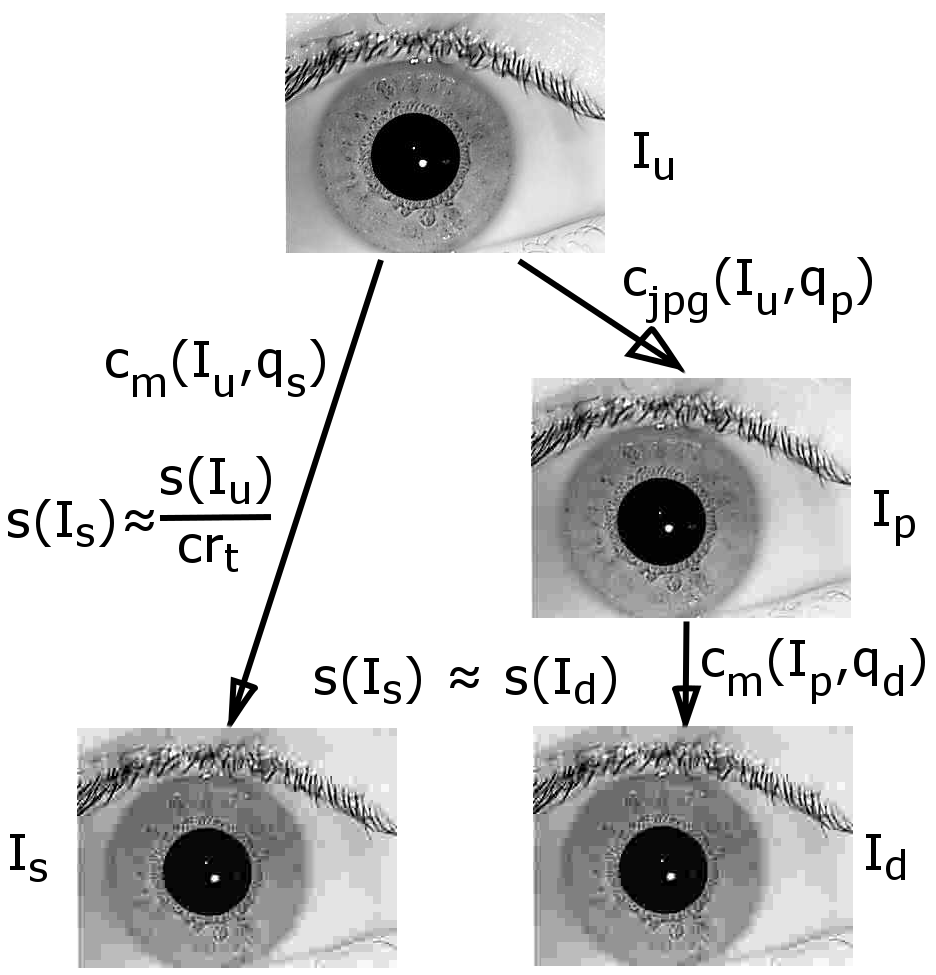
\includegraphics[width=0.7\linewidth]{img/comprScheme}
\end{center}
	\caption{Basic compression principle to obtain two images achieving approximately the same target compression ratio $cr_t$ from an uncompressed image $I_u^{(k)}$ using a particular compression method $m$. One image, $I_s^{(k)}$, is compressed in a single step while the other, $I_d^{(k)}$, uses a pre-compression and a final compression step. Note the pre-compression step is always a $jpg$-compression, while the final compression step uses the same method $m$ as used in the single-compression.}
	\label{fig:comprScheme}
	
\end{figure}

\begin{enumerate}
	\item Compute the single-compressed image $I_s^{(k)}$ with method $m$ such that $cr(I_u^{(k)}, I_s^{(k)}) \approx cr_t$. The optimal quality parameter $q_s^{(k)}$ is computed for each image separately by solving
	\begin{eqnarray}
	\small
	s_t^{(k)} = \frac{s(I_u^{(k)})}{cr_t} \\
		q_s^{(k)} = \underset{q \in \mathbb{N}}{argmin}|s(c_m(I_u^{(k)},q)) - s_t^{(k)}|,
	\end{eqnarray} where $s_t^{(k)}$ is the file size to meet the target compression ratio $cr_t$. This is implemented by iteratively searching for the quality parameter $q$ that results in the compression ratio $cr(I_u, I_c)$ closest to $cr_t$. 
	\item The single compressed images $I_s^{(k)}$ with method $m$ are then computed with the found optimal parameters as
	\begin{equation}
	I_s^{(k)} = c_m(I_u^{(k)}, q_s^{(k)})
	\end{equation}
	
	\item Compute a pre-compressed image $I_p^{(k)}$ representing images in pre-compressed data set. This is done using $jpg$-method \cite{jpg} with an arbitrary but fixed quality parameter $q_p$. Note that pre-compressed images of one data set may have significant varying file sizes depending on the image's content.
	
	\item Now, find a quality parameter $q_d^{(k)}$ that allows to compress the pre-compressed image $I_p^{(k)}$ a second time, such that the resulting double-compressed image $I_d^{(k)}$ has the same file size as the single-compressed image $I_s^{(k)}$, i.e. $s(I_s^{(k)}) \approxeq s(I_d^{(k)})$. Such a quality parameter can be found by optimizing
	\begin{equation}
	\small
		q_d^{(k)} = \underset{q \in \mathbb{N}}{argmin}|s(c_m(I_p^{(k)},q)) - s(I_s^{(k)})| \quad \forall s(I_s^{(k)}) \geq s(I_d^{(k)})
	\end{equation}
	
	The condition $s(I_s^{(k)}) \geq s(I_d^{(k)})$ is of importance to establish fair conditions, since it is very likely that the size cannot be equalized due to the limited universe of the quality parameters of the used compression methods $m$.
	
	\item The double-compressed images $I_d^{(k)}$ are then computed from the pre-compressed images $I_p^{(k)}$ with the found optimal parameters as
	\begin{equation}
		I_d^{(k)} = c_m(I_p^{(k)}, q_d^{(k)})
	\end{equation}
	
\end{enumerate}

\section{Experimental setup}
Although there are several iris data sets around, few are available in uncompressed format. We use the IITD Iris data base\footnote{IITD Iris Database version 1.0, http://www4.comp.polyu.edu.hk/\textasciitilde csajaykr/IITD/Database\_Iris.htm}. The main reason for this is the availability of a segmentation ground truth created by an expert, which was recently introduced by Rathgeb \etal in \cite{severeCompression}. The $k^{th}$ image of this segmentation ground truth data set is subsequently denoted as $SGT^{(k)}$. They also propose segmentation error results compareable to those we define in equation (\ref{equ:mserabs}).
We want to point out that although it is claimed that the data set is in uncompressed BMP format (backed by \cite{severeCompression}), visual evaluation suggests there are block artefacts contained, potentially employed by compression. Although this is the case, using this data set was necessary due to the available ground truth, for reasons discussed in section \ref{section:ser}   %TODO Can we write it this way? Does this void the complete results?!

We use the scheme introduced in section \ref{section:comprScheme} and compress the data for the following set of target compression ratios:
\begin{equation}
cr_t \in \{5,10,15,20,25,30,35,40,50,60,75\}
\end{equation}
For each of these target compression ratios $cr_t$, the pre-compression step in double-compression mode is carried out with the quality parameters
\begin{equation}
q_p \in \{100, 85, 75, 70\}
\end{equation} 
in order to simulate different levels of pre-compression. Each of these combinations is used to compress with the introduced $jpg$, $j2k$ and $jxr$ methods. This results in a total of 165 data sets with 2240 images each.

\textbf{TODO: Statistics of compression accuracy (mean) and stddev}.

This test data set is used to test six implementations of iris recognition algorithms available in the University of Salzburg Iris Toolbox USIT \cite{rathgeb}. 

%TODO should we discuss used methods, i.e. GIMP for converting from JXR to PNG?


\section{Evaluation}
 Besides assessing the image quality with fully-referenced metrics, we investigate the behaviour of segmentation error rate and the system's EER in respect to the compression ratio.


\subsection{Full-referenced quality metrics}
Todo Lefteris:
\begin{itemize}
 \item Which quality metrics were in the selection
 \item Which were chosen
 \item Why have you chosen these
 \item Give a very very brief introduction (rather referencing!) of what the quality metrics are about and the most characteristic features
 \item Results and findings of this evaluation
\end{itemize}

\subsection{Segmentation error rates}
\label{section:ser}
The segmentation of an iris image is by nature a critical part in the process. We investigate the differences of single- and double compression as well as the aspects of using an absolute reference, e.g. a ground truth, or a relative one, e.g. the segmentation of the uncompressed images $I_u$.

\begin{figure}
\begin{center}

  
\includegraphics[width=0.3\linewidth]{img/segMasks/gt.png}
  
\includegraphics[width=0.3\linewidth]{img/segMasks/jpg_caht_q100_cr5.png}
  
\includegraphics[width=0.3\linewidth]{img/segMasks/jpg_wahet_q100_cr5.png}
  \end{center}
  
  \label{fig:segMasks}
  \caption{Segmentation masks of the expert ground truth \cite{severeCompression}, relative groundtruth $seg(I_u^{(k)})$ and an actual segmentation result $seg(I_d^{(k)})$ (f.l.t.r)}
\end{figure}

%TODO discuss, why the eye lashes are notmasked in the algos


The segmentation accuracy is rated by the mean segmentation error rate, which corresponds to the suggested E1 error rate in the Noisy Iris Challenge Evaluation - Part I (NICE.I), also used in \cite{severeCompression}. We define the segmentation error rate $ser$ of a single image $I$ as
\begin{equation}
ser(R,S) = \overline{R \oplus S} \in [0,1]\quad with \quad R,S \in \{0,1\}^{w \times h},
\end{equation} where $R$ is the binarized reference segmentation and $S$ the binarized segmentation result of the same image $I$. The mean value of the pixel-wise exclusive-or is the percentage of pixels different in the segmented image $S$ in respect to the reference $R$. Due to multiple images in a data base, the mean segmentation error $mser$ is computed from $K$ images. In this experiment, we compute error rates for the single- and double compressed images $I_c \in {I_s, I_d}$. We define the absolute mean segmentation error $mser_{abs}$ in respect to the ground truth $SGT$ from \cite{severeCompression} and the relative mean segmentation error $mser_{rel}$ in respect to the segmentation of the uncompressed images $I_u$. By denoting the segmentation process of an image $I$ as $seg(I) \in \{0,1\}^{w \times h}$ we have
\begin{eqnarray}
mser_{abs} = \frac{1}{K}\sum_{k=1}^{K}ser(SGT^{(k)},seg(I_c^{(k)})) \label{equ:mserabs} \\
mser_{rel} = \frac{1}{K}\sum_{k=1}^{K}ser(seg(I_u^{(k)}),seg(I_c^{(k)})) \label{equ:mserrel} \\
\end{eqnarray}

The absolute segmentation error rate, hence also the development in respect to compression ratio can be considered to be optimal because of the available ground truth. However, for most data bases no such ground truth is available. therefore we evaluate if a corresponding conclusion can be withdrawn from the relative segmentation error $mser_{rel}$ as well. The benefit of such a relation is that the $mser_{rel}$ can be computed for any arbitrary data set easily. 

\begin{figure}[h]
	\begin{center}
		
	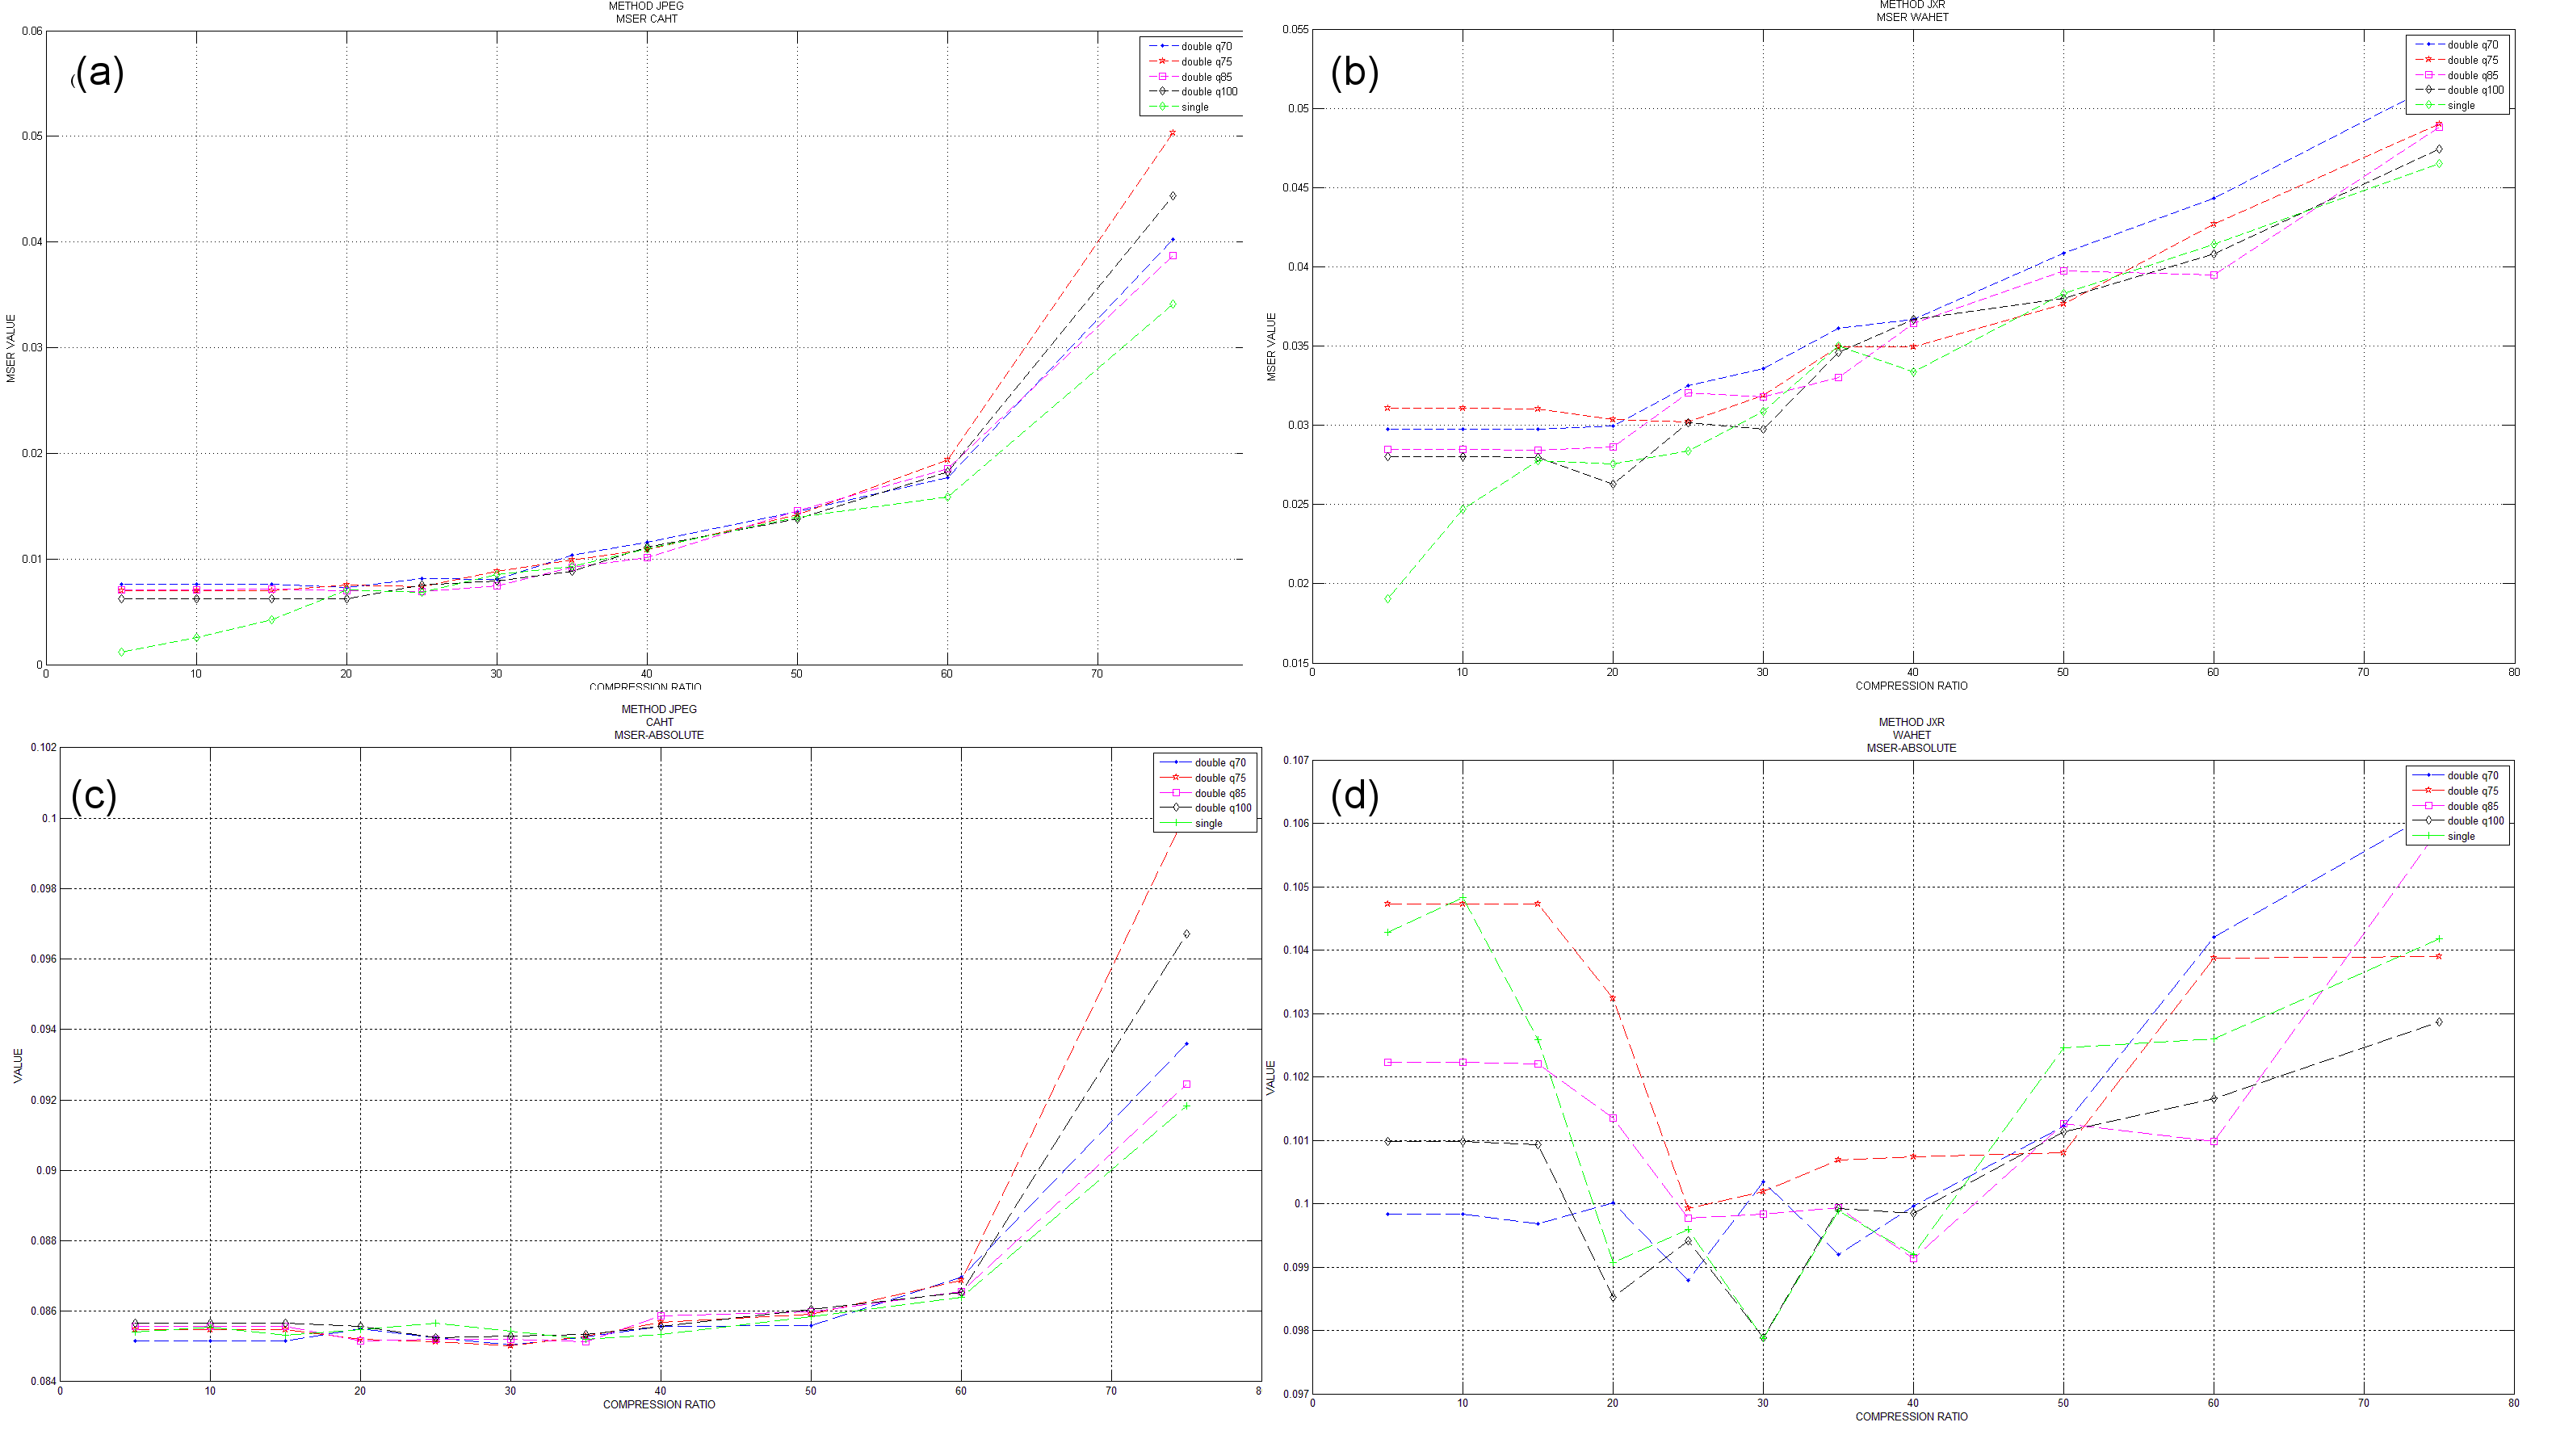
\includegraphics[width=\linewidth]{img/segResults}
\end{center}
	\caption{Top: Relative segmentation results with CAHT on $jpg$-compressed (a) and WAHET on $jxr$-compressed data (b). Bottom: Absolute segmentation results (c) and (d) with the same methods as in (a) and (b).}
	\label{fig:segResults}
	
\end{figure}

The experiments were carried out for CAHT and WAHET segmentation \cite{rathgeb}. From the graphs in Figure \ref{fig:segResults} we observe that

\begin{itemize}
 \item there is no significant difference in segmenting single-compressed or double-compressed images for medium compression ratios, i.e. $ 20 \leq cr_t \leq 50 $,
 \item there is a difference for small compression ratios, i.e. $cr_t < 20$, and large compression ratios, i.e. $cr_t > 50$. However, there is no trend in segmentation accuracy observeable, when investigating the difference between the single- or the double-compressed images and% TODO rephrase
 \item the $mser_{abs}$ is generally higher than $mser_{rel}$, because the segmentation algorithms ignore eyelids, yet are considered in the expert ground truth \cite{severeCompression}.
 \item Comparing $mser_{rel}$ and $mser_{abs}$ indicates that in most cases both metrics show the same characteristics, especially for medium and large compression ratios, i.e. $cr_t > 20$. For the WAHET segmentation, however, the results obtained with $jxr$ and $j2k$ compressed data contradict this observation. Hence, in a general case a ground truth is indeed needed to investigate the impact of compression on iris segmentation algorithms. Since this was concluded from two segmentation methods only, further investigation is necessary for this aspect.
\end{itemize}




TODO TB:
\begin{itemize}
 \item Transform CR's in bpp, compare to \cite{severeCompression}
\end{itemize}


\subsection{Equal Error rate}
To assess the total impact on the System, the EER is computed
TODO TB

\begin{itemize}
 \item Brief introduction
 \item Results and findings of this evaluation
\end{itemize}


\section{Results}
\subsection{Schnoell-Correlation-method}
TODO: Martin: Introduce your method here and argue why it is better than spearman

\subsection{Correlation of Evaluation methods}
TODO: Martin:
Provide sensible correlation results and analyse


\section{Conclusion}
TODO: Martin Schnöll


{\small
\bibliographystyle{ieee}
\bibliography{egbib}
}

\end{document}
